\documentclass[12pt, letter]{article}

\usepackage[margin=0.8in]{geometry}
\usepackage{amssymb}
\usepackage{amsmath}
\usepackage{tikz}

\title{CS 381 - A2}
\author{Martin Mueller}
\date{Due: Friday, February $21^{st}$, 2020}

\begin{document}
	\maketitle
	\begin{enumerate}
		\item (7 points) Show that the set of all strings $x \in \{0, 1\}^*$, such that $x$ is either a multiple of $3$ or $x$ is a multiple of $5$, is regular. Give a digitally-drawn state diagram that is well-organized and the states have intuitive yet concise labels. Give a concise and precise English description of how your DFA works. Finally, give a formal description of your DFA, contained in the file A2-1.dfa, that runs in the Automata-Simulator.
		\begin{center}
			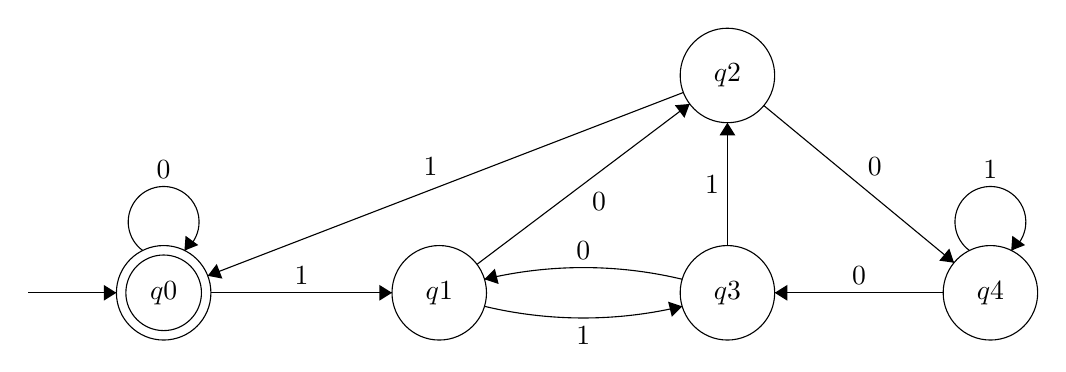
\begin{tikzpicture}[scale=0.2]
				\tikzstyle{every node}+=[inner sep=0pt]
				\draw [black] (16.6,-22.7) circle (3);
				\draw (16.6,-22.7) node {$q0$};
				\draw [black] (16.6,-22.7) circle (2.4);
				\draw [black] (34.1,-22.7) circle (3);
				\draw (34.1,-22.7) node {$q1$};
				\draw [black] (52.4,-8.9) circle (3);
				\draw (52.4,-8.9) node {$q2$};
				\draw [black] (52.4,-22.7) circle (3);
				\draw (52.4,-22.7) node {$q3$};
				\draw [black] (69.1,-22.7) circle (3);
				\draw (69.1,-22.7) node {$q4$};
				\draw [black] (19.6,-22.7) -- (31.1,-22.7);
				\fill [black] (31.1,-22.7) -- (30.3,-22.2) -- (30.3,-23.2);
				\draw (25.35,-22.2) node [above] {$1$};
				\draw [black] (36.5,-20.89) -- (50,-10.71);
				\fill [black] (50,-10.71) -- (49.06,-10.79) -- (49.67,-11.59);
				\draw (44.25,-16.3) node [below] {$0$};
				\draw [black] (54.71,-10.81) -- (66.79,-20.79);
				\fill [black] (66.79,-20.79) -- (66.49,-19.89) -- (65.85,-20.66);
				\draw (61.76,-15.31) node [above] {$0$};
				\draw [black] (15.277,-20.02) arc (234:-54:2.25);
				\draw (16.6,-15.45) node [above] {$0$};
				\fill [black] (17.92,-20.02) -- (18.8,-19.67) -- (17.99,-19.08);
				\draw [black] (8,-22.7) -- (13.6,-22.7);
				\fill [black] (13.6,-22.7) -- (12.8,-22.2) -- (12.8,-23.2);
				\draw [black] (67.777,-20.02) arc (234:-54:2.25);
				\draw (69.1,-15.45) node [above] {$1$};
				\fill [black] (70.42,-20.02) -- (71.3,-19.67) -- (70.49,-19.08);
				\draw [black] (49.6,-9.98) -- (19.4,-21.62);
				\fill [black] (19.4,-21.62) -- (20.33,-21.8) -- (19.97,-20.87);
				\draw (33.55,-15.28) node [above] {$1$};
				\draw [black] (36.973,-21.84) arc (103.47443:76.52557:26.941);
				\fill [black] (36.97,-21.84) -- (37.87,-22.14) -- (37.63,-21.17);
				\draw (43.25,-20.6) node [above] {$0$};
				\draw [black] (52.4,-19.7) -- (52.4,-11.9);
				\fill [black] (52.4,-11.9) -- (51.9,-12.7) -- (52.9,-12.7);
				\draw (51.9,-15.8) node [left] {$1$};
				\draw [black] (66.1,-22.7) -- (55.4,-22.7);
				\fill [black] (55.4,-22.7) -- (56.2,-23.2) -- (56.2,-22.2);
				\draw (60.75,-22.2) node [above] {$0$};
				\draw [black] (49.527,-23.559) arc (-76.53718:-103.46282:26.963);
				\fill [black] (49.53,-23.56) -- (48.63,-23.26) -- (48.87,-24.23);
				\draw (43.25,-24.8) node [below] {$1$};
			\end{tikzpicture}
			\newline
			The above DFA determines if a given binary string is divisible by 5. It does so by processing the remainder of the string. Each state $q_{n}$ represents the remainder $n$ of the given string divided by $5$. Any string with a remainder of $0$ when divided by $5$ is, by definition, divisible by $5$. \\
			From this DFA, we can gather that the language $\{x | x \text{ is a multiple of 5}\}$ is regular. We also know from a DFA derived in class that the language $\{x | x \text{ is a multiple of 3}\}$ is regular. We can now use these two DFAs to derive the above language. Also discussed and proved in class was that the class of regular languages is closed under the union operation. If we take the union of the language of the DFA derived in class with the language of the DFA above, we can obtain the language $\{x | x \text{ is either a multiple of 3 or a multiple of 5}\}$. Since this language can be obtained through a union of two regular languages, it stands to reason that this language is also regular.
		\end{center}
	\item (13 points) Let $A$ and $B$ be languages comprised of binary strings. Define the following "implication" operator $\rightarrow$ on sets as follows: $A \rightarrow B = \left\{ x \mid x \in A \rightarrow x \in B \right\}$. Show that the class of regular languages is closed under implication. In other words, if $A_1$ and $A_2$ are regular languages, then so is $A_1 \rightarrow A_2$. Your construction must be deterministic. Give a full construction, the level of detail of which should be similar to the level of detail we used in class to show that the class of regular languages is closed under union. Also, give a concise and precise English description of your proof "strategy" or "idea" so I can get a good sense of what you're doing.
	\end{enumerate}
	\begin{center}
		I will be using definitions of logical operators and DFAs to show it is possible to construct a regular language from $A \rightarrow B$ provided $A$ and $B$ are regular languages. Let us start with first rewriting the implication operator definition:
		\begin{align*}
			A \rightarrow B &= \{x \mid x \in A \rightarrow x \in B\} \\
			&= \{x \mid \neg (x \in A) \vee (x \in B)\} \\
			&= \{x \mid x \not\in A\} \cup \{x \mid x \in B\} \\
			&= \neg A \cup B
		\end{align*}
		From this simplification, we can gather two things: One, we know that $B$ is a regular language by the definition of the implication operator, and two, since the union of two regular languages results in a regular language, if $\neg A$ is regular, then the class of regular languages is closed under the implication operator. To prove that $\neg A$ is a regular language, let's construct a DFA that recognizes $\neg A$. We'll start by constructing a DFA $M$ that recognizes $A$:
		\begin{align*}
			M &= (Q, \Sigma^{*}, \delta, q_{0}, F) \\
			Q &= \text{the set of all the states of } M \\
			\Sigma^{*} &= \{0, 1\}^{*} \\
			\delta &= \text{the transition function of } M \\
			q_{0} &= \text{the start state} \\
			F &= \text{the set of all accept states of } M
		\end{align*}
		From this, we can construct $M'$, a machine that recognizes the language $\neg A$. If $A$ is the set of all strings $M$ accepts, then $\neg A$ is the set of all strings that $M$ doesn't accept. This is simply all the states of $M$ that aren't in $F$, or $Q - F$. Using this, we can construct $M'$: $M' = (Q, \Sigma^{*}, \delta, q_{0}, Q - F)$. Since we are able to construct a DFA $M'$ that recognizes the language $\neg A$, the language $\neg A$ is regular, and therefore, since $B$ is also regular and the class of regular languages is closed under the union operation, the class of regular languages is also closed under the implication operation.
	\end{center}
	\vfill \hfill Submit your PDF (generated from \LaTeX) and DFA files in one ZIP file. 
\end{document}